\documentclass[12pt]{report}
\usepackage[utf8x]{inputenc}
\usepackage[russian]{babel}
\usepackage{listings}
\usepackage{graphicx}
\usepackage{amsmath,amsfonts,amssymb,amsthm,mathtools}
\usepackage{pgfplots}
\usepackage{filecontents}
\usepackage{indentfirst}
\usepackage{eucal}
\usepackage{float}
\usepackage{caption}
\usepackage{enumitem}
\usepackage{multirow}
\frenchspacing


% Для листинга кода:
\lstset{ %
language=c,
extendedchars=\true,     % выбор языка для подсветки (здесь это С)
basicstyle=\small\sffamily, % размер и начертание шрифта для подсветки кода
numbers=left,               % где поставить нумерацию строк (слева\справа)
numberstyle=\tiny,           % размер шрифта для номеров строк
stepnumber=1,                   % размер шага между двумя номерами строк
numbersep=5pt,                % как далеко отстоят номера строк от подсвечиваемого кода
showspaces=false,            % показывать или нет пробелы специальными отступами
showstringspaces=false,      % показывать или нет пробелы в строках
showtabs=false,             % показывать или нет табуляцию в строках
frame=single,              % рисовать рамку вокруг кода
tabsize=2,                 % размер табуляции по умолчанию равен 2 пробелам
captionpos=t,              % позиция заголовка вверху [t] или внизу [b]
breaklines=true,           % автоматически переносить строки (да\нет)
breakatwhitespace=false, % переносить строки только если есть пробел
escapeinside={\#*}{*)},   % если нужно добавить комментарии в коде
}


\usepackage[left=3cm,right=1cm, top=2cm,bottom=2cm,bindingoffset=0cm]{geometry}
% Для измененных титулов глав:
\usepackage{titlesec, blindtext, color} % подключаем нужные пакеты
\definecolor{gray75}{gray}{0.75} % определяем цвет
\newcommand{\hsp}{\hspace{20pt}} % длина линии в 20pt
% titleformat определяет стиль
\usepackage{titlesec}

\lstdefinestyle{mystyle}{
    language=Lisp,
	backgroundcolor=\color{white},
	basicstyle=\footnotesize\ttfamily,
	keywordstyle=\color{blue},
	stringstyle=\color{red},
	commentstyle=\color{gray},
	directivestyle=\color{orange},
	numbers=left,
	numberstyle=\tiny,
	stepnumber=1,
	numbersep=5pt,
	frame=single,
	tabsize=4,
	captionpos=t,
	breaklines=true,
	breakatwhitespace=true,
	escapeinside={\#*}{*)},
	morecomment=[l][\color{magenta}]{\#},
	columns=fullflexible
}

\lstset{style=mystyle}

\titleformat{\section}[block]
{\Large\filcenter\newpage\MakeUppercase}
  {\thesection}
  {1em}
  {\MakeUppercase}{}

\linespread{1.25}
\setlength\parindent{5ex}

\begin{document}
\thispagestyle{empty}
\begin{titlepage}
	\noindent \begin{minipage}{0.15\textwidth}
	
\includegraphics[width=\linewidth]{./images/b_logo.jpg}
	\end{minipage}
	\noindent\begin{minipage}{0.9\textwidth}\centering
		\textbf{Министерство науки и высшего образования Российской Федерации}\\
		\textbf{Федеральное государственное бюджетное образовательное учреждение высшего образования}\\
		\textbf{«Московский государственный технический университет имени Н.Э.~Баумана}\\
		\textbf{(национальный исследовательский университет)»}\\
		\textbf{(МГТУ им. Н.Э. Баумана)}
	\end{minipage}

	\noindent\rule{18cm}{3pt}
	\newline\newline
	\noindent ФАКУЛЬТЕТ $\underline{\text{«Информатика и системы управления»}}$ \newline\newline
	\noindent КАФЕДРА $\underline{\text{«Программное обеспечение ЭВМ и информационные технологии»}}$\newline\newline\newline\newline\newline

  \begin{center}
        \Large\textbf{Отчет по лабораторной работе №1 по курсу "Математическая статистика"}
    \end{center}

	\noindent\textbf{Тема} $\underline{\text{Гистограмма и эмпирическая функция распределения}}$\newline\newline
	\noindent\textbf{Студент} $\underline{\text{Пантелеев В.М.}}$\newline\newline
	\noindent\textbf{Группа} $\underline{\text{ИУ7-62Б}}$\newline\newline
	\noindent\textbf{Оценка (баллы)} $\underline{\text{~~~~~~~~~~~~~~~~~~~~~~~~~~~}}$\newline\newline
	\noindent\textbf{Преподаватели} $\underline{\text{Власов П.А.}}$\newline\newline\newline

	\begin{center}
		\vfill
		Москва~---~\the\year
		~г.
	\end{center}
\end{titlepage}

\renewcommand{\thefigure}{\thesection.\arabic{figure}}
\renewcommand{\thetable}{\thesection.\arabic{table}}
\renewcommand{\thelstlisting}{\thesection.\arabic{lstlisting}}


\renewcommand*\thesection{\arabic{section}}


\section{Задание}

\textbf{Цель работы:} построение гистограммы и эмпирической функции распределения.

\textbf{Содержание работы:}
\begin{enumerate}
    \item Для выборки объёма $n$ из генеральной совокупности $X$ реализовать в виде программы на ЭВМ
        \begin{enumerate}
            \item вычисление максимального значения $M_{\max}$ и минимального значения $M_{\min}$;
            \item размаха $R$ выборки;
            \item вычисление оценок $\hat\mu$ и $S^2$ математического ожидания $MX$ и дисперсии $DX$;
            \item группировку значений выборки в $m = [\log_2 n] + 2$ интервала;
            \item построение на одной координатной плоскости гистограммы и графика функции плотности распределения вероятностей нормальной случайной величины с математическим ожиданием $\hat{\mu}$ и дисперсией $S^2$;
            \item построение на другой координатной плоскости графика эмпирической функции распределения и функции распределения нормальной случайной величины с математическим ожиданием $\hat{\mu}$ и дисперсией $S^2$.
        \end{enumerate}
    \item Провести вычисления и построить графики для выборки из индивидуального варианта.
\end{enumerate}

\section{Теоретические сведения}

\subsection{Формулы для вычисления величин}

\subsubsection{Минимальное и максимальное значения выборки}
\begin{equation}
    \begin{aligned}
        M_{\max} = X_{(n)}\\
        M_{\min} = X_{(1)}
    \end{aligned}
\end{equation}

\subsubsection{Размах выборки}
\begin{equation}
    R = M_{\max} - M_{\min}.
\end{equation}

\subsubsection{Оценки математического ожидания и исправленной дисперсии}
\begin{equation}
    \begin{aligned}
    \hat\mu(\vec X_n) &= \frac 1n \sum_{i=1}^n X_i\\
    S^2(\vec X_n) &= \frac 1{n-1} \sum_{i=1}^n (X_i-\overline X_n)^2
    \end{aligned}
\end{equation}

\section{Определение эмпирической плотности и гистограммы}

Пусть $\vec x$ -- выборка из генеральной совокупности $X$. Если объем $n$ этой выборки велик, то значения $x_i$ группируют в интервальный статистический ряд. Для этого отрезок $J = [x_{(1)}, x_{(n)}]$ делят на $m$ равновеликих частей:

\begin{equation*}
    J_i = [x_{(1)} + (i - 1) \cdot \Delta, x_{(1)} + i \cdot \Delta), i = \overline{1; m - 1},
\end{equation*}

\begin{equation*}
    J_{m} = [x_{(1)} + (m - 1) \cdot \Delta, x_{(n)}],
\end{equation*}

\begin{equation*}
    \Delta = \frac{|J|}{m} = \displaystyle\frac{x_{(n)} - x_{(1)}}{m}.
\end{equation*}

Интервальным статистическим рядом называют таблицу:

\begin{table}[htb]
    \centering
    \begin{tabular}{|c|c|c|c|c|}
        \hline
        $J_1$ & ... & $J_i$ & ... & $J_m$ \\
        \hline
        $n_1$ & ... & $n_i$ & ... & $n_m$ \\
        \hline
    \end{tabular}
\end{table}

где $n_i$ -- количество элементов выборки $\vec x$, которые $\in J_i$.

Обычно выборку разбивают на $m=[\log_2n]+2$ интервалов, где $n$ -- размер выборки.

\textit{Эмпирической плотностью}, отвечающей выборке $\vec x$, называют функцию:
\begin{equation}
    \hat f(x) =
    \begin{cases}
        \displaystyle\frac{n_i}{n \Delta}, \quad x \in J_i, i = \overline{1; m}, \\
        0, \quad \text{ иначе,} \\
    \end{cases}
\end{equation}
где $J_i$ -- полуинтервал статистического ряда, $n_i$ -- количество элементов выборки, входящих в полуинтервал, $n$ -- количество элементов выборки.

Гистограмма -- это график эмпирической плотности.

\section{Определение эмпирической функции распределения}

Пусть $\vec x = (x_1, ..., x_n)$ -- выборка из генеральной совокупности $X$. Обозначим $n(x, \vec x)$ -- число элементов вектора $\vec x$, которые имеют значения меньше $x$.

\textit{Эмпирической функцией распределения} называют функцию $F_n: \mathbb{R} \to \mathbb{R}$, определенную как:

\begin{equation}
    F_n(x) = \frac{n(x, \vec x)}{n}.
\end{equation}

Замечание.
\begin{enumerate}
    \item  Обладает всеми свойствами функции распределения;
    \item  Кусочно-постоянна;
    \item Если все элементы вектора различны, то

    \begin{equation}
    F(x) =
    \begin{cases}
    0, \quad x \leq x_{(1)}, \\
        \displaystyle\frac{i}{n}, \quad x_{(i)} < x \leq  x_{(i+1)},\\
        1, \quad  x > x_{(n)}. \\
    \end{cases}.
\end{equation}
\end{enumerate}

\section{Результат работы}

Вариант 12

\subsection{Код программы}

\begin{lstlisting}
function lab_1()
    function [amnt] = count_less(t, X)
        tol = 1e-4;
        amnt = 0;
        for x_index = 1:length(X)
            if (X(x_index) - t < tol)
                amnt = amnt + 1;
            end
        end
    end

    X = [11.89,9.60,9.29,10.06,9.50,8.93,9.58,6.81,8.69,9.62,...
        9.01,10.59,10.50,11.53,9.94,8.84,8.91,6.90,9.76,7.09,...
        11.29,11.25,10.84,10.76,7.42,8.49,10.10,8.79,11.87,...
        8.77,9.43,12.41,9.75,8.53,9.72,9.45,7.20,9.23,8.93,...
        9.15,10.19,9.57,11.09,9.97,8.81,10.73,9.57,8.53,9.21,...
        10.08,9.10,11.03,10.10,9.47,9.72,9.60,8.21,7.78,10.21,...
        8.99,9.14,8.60,9.14,10.95,9.33,9.98,9.09,10.35,8.61,...
        9.35,10.04,7.85,9.64,9.99,9.65,10.89,9.08,8.60,7.56,...
        9.27,10.33,10.09,8.51,9.86,9.24,9.63,8.67,8.85,11.57,...
        9.85,9.27,9.69,10.90,8.84,11.10,8.19,9.26,9.93,10.15,...
        8.42,9.36,9.93,9.11,9.07,7.21,8.22,9.08,8.88,8.71,...
        9.93,12.04,10.41,10.80,7.17,9.00,9.46,10.42,10.43,8.38,9.01];

    X = sort(X);

    m_max = max(X);
    m_min = min(X);

    fprintf("\n1)M_max = %f.\n  M_min = %f.\n\n", m_max, m_min);

    R = m_max - m_min;
    fprintf("\n2)Размах выборки: R = %f.\n\n", R);


    n = length(X);
    q = sum(X) / n;
    S2 = sum((X - q).^2) / (n - 1);
    fprintf("\n3)q = %f.\n", q);
    fprintf("S^2 = %f.\n", S2);

    m = floor(log2(n)) + 2;
    groups = [];
    curr = m_min;
    d = R / m;

    for i = 1:(m + 1)
        groups(i) = curr;
        curr = curr + d;
    end

    eps = 1e-6;
    amounts = [];

    tot = 0;

    for i = 1:(m - 1)
        curr = 0;

        for j = 1:n
            if ((X(j) - groups(i)) > eps || abs(groups(i) - X(j)) < eps) && (X(j) - groups(i + 1) < eps)
                curr = curr + 1;
            end
        end

        amounts(i) = curr;
        tot = tot + curr;
    end

    amounts(m) = n - tot;

    fprintf("\n4)Группировка значений выборки  в %d интервалов:\n", m);
    for i = 1:(m)
        fprintf("Интервал %d [%f : %f) - %d значений из выборки.\n", i, groups(i), groups(i + 1), amounts(i));
    end


    fprintf("\n5)Построение гистограммы и графика функции плотности распределения нормальной случайной величины.\n");
    figure;
    hold on;
    grid on;

    cent = zeros(1, m);
    heights = zeros(1, m);

    for i = 1:m
        heights(i) = amounts(i) / (n * d);
    end

    for i = 1:m
        cent(i) = groups(i + 1) - (d / 2);
    end

    set(gca, "xtick", groups);
    set(gca, "ytick", unique(sort(heights)));
    set(gca, "xlim", [min(groups) - 1, max(groups) + 1]);

    bar(cent, heights, 1);
    points = (m_min - 5):(S2 / 250):(m_max + 5);
    X_pdf = normpdf(points, q, sqrt(S2));
    plot(points, X_pdf, "r", 'LineWidth', 2);

    xlabel('x')
    ylabel('f(x)')
    hold off;

    fprintf("\n6)Построение графика эмпирической функции распределения и функции распределения нормальной случайной величины.\n");
    figure;
    hold on;
    grid on;

    x = unique(X);
    x(end + 1) = x(end) + 1;
    heights = zeros([1 length(x)]);
    for i = 1:length(x)
        heights(i) = count_less(x(i), X) / n;
    end

    heightss = unique(heights);

    set(gca, "ylim", [0, max(heightss) + 0.3]);
    stairs(x, heights);

    points = (m_min - 2):(S2 / 250):(m_max + 2);
    x_cdf = normcdf(points, q, sqrt(S2));
    plot(points, x_cdf, "r");

    xlabel('x')
    ylabel('F(x)')
    hold off;
end

\end{lstlisting}

\section{Результаты расчётов}

\begin{equation*}
M_{\min} = 6.81 \\
\end{equation*}
\begin{equation*}
M_{\max} = 12.41 \\
\end{equation*}
\begin{equation*}
    R = 5.60 \\
\end{equation*}
\begin{equation*}
    \hat\mu(\vec x_n) = 9.487 \\
\end{equation*}
\begin{equation*}
    S^2(\vec x_n) = 1.217 \\
\end{equation*}
\begin{equation*}
    m = 8
\end{equation*}

Группировка значений выборки в 8 интервалов:
\begin{itemize}
    \item интервал 1 [6.810000 : 7.510000) - 7 значений из выборки;
    \item интервал 2 [7.510000 : 8.210000) - 5 значений из выборки;
    \item интервал 3 [8.210000 : 8.910000) - 22 значений из выборки;
    \item интервал 4 [8.910000 : 9.610000) - 36 значений из выборки;
    \item интервал 5 [9.610000 : 10.310000) - 27 значений из выборки;
    \item интервал 6 [10.310000 : 11.010000) - 14 значений из выборки;
    \item интервал 7 [11.010000 : 11.710000) - 7 значений из выборки;
    \item интервал 8 [11.710000 : 12.410000) - 2 значений из выборки.
\end{itemize}

\newpage
\begin{figure}[H]
	\begin{center}
		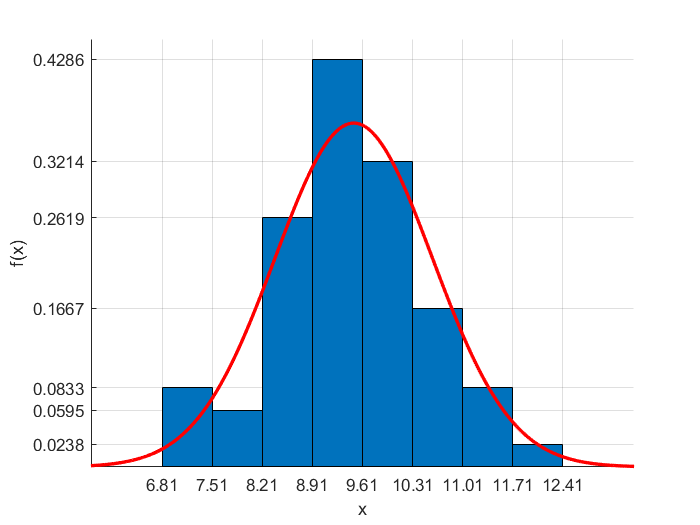
\includegraphics[scale=0.6]{./images/2.png}
			\caption{Гистограмма и график функции плотности распределения вероятностей нормальной случайной величины с выборочными мат. ожиданием и дисперсией.}
	\end{center}
	\label{img:eval}
\end{figure}


\begin{figure}[H]
	\begin{center}

		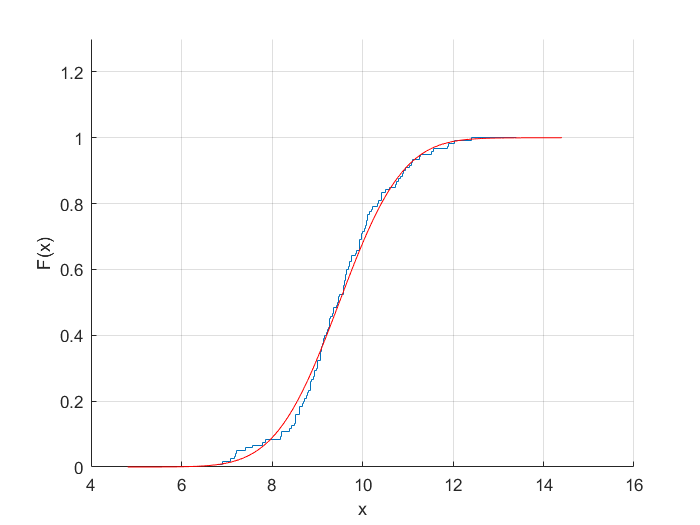
\includegraphics[scale=0.6]{./images/1.png}
			\caption{График эмпирической функции распределения и функции распределения нормальной случайной величины с выборочными мат. ожиданием и дисперсией.}
	\end{center}
	\label{img:eval}
\end{figure}


\end{document}